\chapter{Recurrent neural networks}


\section{Architectures}


\subsection{(Elman) recurrent neural network}

\begin{description}
    \item[Recurrent neural network (RNN)] \marginnote{Recurrent neural network (RNN)}
        Neural network that processes a sequential input. At each iteration, an input is fed to the network and the hidden activation is computed considering both the input and the hidden activation of the last iteration.

        \begin{figure}[H]
            \centering
            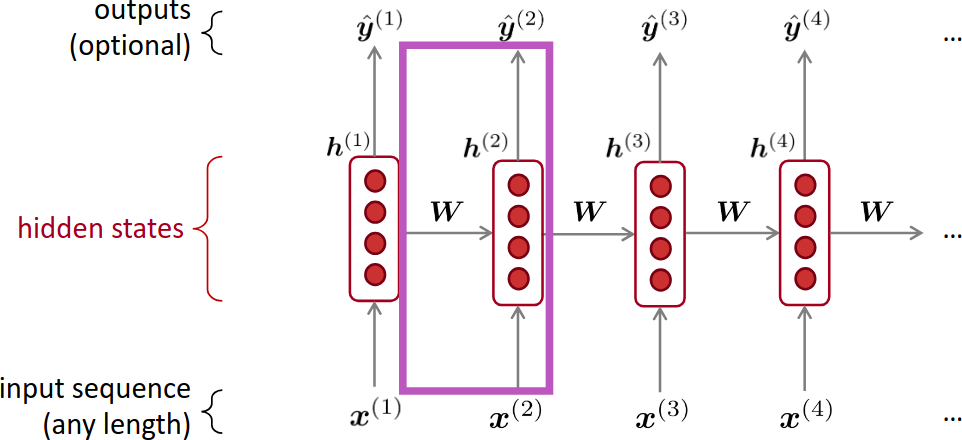
\includegraphics[width=0.5\linewidth]{./img/rnn_unrolled.png}
            \caption{RNN unrolled in time}
        \end{figure}

    \item[RNN language model (RNN-LM)] \marginnote{RNN language model (RNN-LM)}
    Given an input word $w^{(t)}$, an RNN-LM does the following:
    \begin{enumerate}
        \item Compute the embedding $\vec{e}^{(t)}$ of $w^{(t)}$.
        \item Compute the hidden state $\vec{h}^{(t)}$ considering the hidden state $\vec{h}^{(t-1)}$ of the previous step:
        \[ \vec{h}^{(t)} = f(\matr{W}_e \vec{e}^{(t)} + \matr{W}_h \vec{h}^{(t-1)} + \vec{b}_1) \]
        \item Compute the output vocabulary distribution $\hat{\vec{y}}^{(t)}$:
        \[ \hat{\vec{y}}^{(t)} = \texttt{softmax}(\matr{U}\vec{h}^{(t)} + \vec{b}_2) \]
        \item Repeat for the next token.
    \end{enumerate}

    \begin{figure}[H]
        \centering
        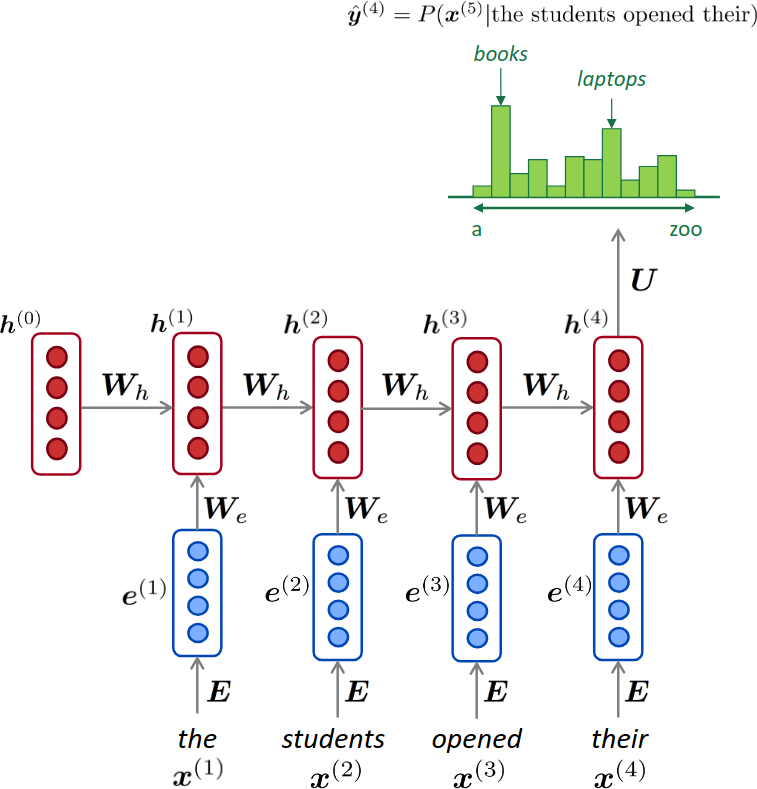
\includegraphics[width=0.4\linewidth]{./img/rnn_lm.png}
    \end{figure}

    \begin{remark}
        RNN-LMs allow to generate the output autoregressively.
    \end{remark}

    \begin{description}
        \item[Training]
            Given the predicted distribution $\hat{\vec{y}}^{(t)}$ and ground-truth $\vec{y}^{(t)}$ at step $t$, the loss is computed as the cross-entropy:
            \[ \mathcal{L}^{(t)}(\matr{\theta}) = - \sum_{v \in V} \vec{y}_v^{(t)} \log\left( \hat{\vec{y}}_v^{(t)} \right) \]

            \begin{description}
                \item[Teacher forcing] \marginnote{Teacher forcing}
                    During training, as the ground-truth is known, the input at each step is the correct token even if the previous step outputted the wrong value.

                    \begin{remark}
                        This allows to stay closer to the ground-truth and avoid completely wrong training steps.
                    \end{remark}
            \end{description}
    \end{description}
\end{description}

\begin{remark}
    RNNs grow in width and not depth, and cannot be parallelized.
\end{remark}


\subsection{Long short-term memory}

\begin{remark}[Vanishing gradient]
    In RNNs, the gradient of distant tokens vanishes through time. Therefore, long-term effects are hard to model.
\end{remark}

\begin{description}
    \item[Long short-term memory (LSTM)] \marginnote{Long short-term memory (LSTM)}
        Architecture where at each step $t$ outputs:
        \begin{descriptionlist}
        \item[Hidden state] $\vec{h}^{(t)} \in \mathbb{R}^{n}$ as in RNNs.
        \item[Cell state] $\vec{c}^{(t)} \in \mathbb{R}^{n}$ with the responsibility of long-term memory.
        \end{descriptionlist}

        \begin{description}
            \item[Gates]
                Non-linear operators to manipulate the cell state (in the following part, $\matr{W}_*$, $\matr{U}_*$, and $\vec{b}_*$ are parameters).

                \begin{description}
                    \item[Forget gate] \marginnote{Forget gate}
                        Controls what part of the cell state to keep:
                        \[ \vec{f}^{(t)} = \sigma\left( \matr{W}_f \vec{h}^{(t-1)} + \matr{U}_f \vec{x}^{(t)} + \vec{b}_f \right) \]

                    \item[Input gate] \marginnote{Input gate}
                        Controls what part of the input to write in the cell state:
                        \[ \vec{i}^{(t)} = \sigma\left( \matr{W}_i \vec{h}^{(t-1)} + \matr{U}_i \vec{x}^{(t)} + \vec{b}_i \right) \]

                    \item[Output gate] \marginnote{Output gate}
                        Controls what part of the cell state to include in the output hidden state:
                        \[ \vec{o}^{(t)} = \sigma\left( \matr{W}_o \vec{h}^{(t-1)} + \matr{U}_o \vec{x}^{(t)} + \vec{b}_o \right) \]
                    \end{description}

                Updates are done as follows:
                \begin{descriptionlist}
                    \item[New cell state content] $\tilde{\vec{c}}^{(t)} = \texttt{tanh}\left( \matr{W}_c \vec{h}^{(t-1)} + \matr{U}_c \vec{x}^{(t)} + \vec{b}_c \right)$.
                    \item[Cell state] $\vec{c}^{(t)} = \vec{f}^{(t)} \cdot \vec{c}^{(t-1)} + \vec{i}^{(t)} \cdot \tilde{\vec{c}}^{(t)}$.
                    \item[Hidden state] $\vec{h}^{(t)} = \vec{o}^{(t)} \cdot \texttt{tanh}(\vec{c}^{(t)})$.
                \end{descriptionlist}
        \end{description}

        \begin{remark}
            LSTMs make it easier to preserve information over time, but they might still be affected by the vanishing gradient problem.
        \end{remark}

        \begin{figure}[H]
            \centering
            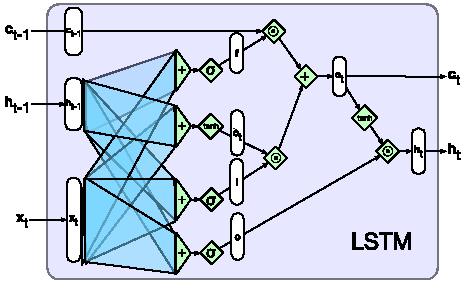
\includegraphics[width=0.5\linewidth]{./img/_lstm.pdf}
        \end{figure}
\end{description}


\subsection{Gated recurrent units}

\begin{description}
    \item[Gated recurrent units (GRU)] \marginnote{Gated recurrent units (GRU)}
        Simpler architecture than LSTMs with fewer gates and without the cell state.

        \begin{description}
            \item[Gates] \phantom{}
                \begin{description}
                    \item[Update gate] \marginnote{Update gate}
                        Controls what part of the current hidden state to keep:
                        \[ \vec{u}^{(t)} = \sigma\left( \matr{W}_u \vec{h}^{(t-1)} + \matr{U}_u \vec{x}^{(t)} + \vec{b}_u \right) \]
        
                    \item[Reset gate] \marginnote{Reset gate}
                        Controls what part of the previous hidden state to use:
                        \[ \vec{r}^{(t)} = \sigma\left( \matr{W}_r \vec{h}^{(t-1)} + \matr{U}_r \vec{x}^{(t)} + \vec{b}_r \right) \]
                \end{description}
        \end{description}

        Updates are done as follows:
        \begin{descriptionlist}
            \item[New hidden state content] $\tilde{\vec{h}}^{(t)} = \texttt{tanh}\left( \matr{W}_h(\vec{r}^{(t)} \cdot \vec{h}^{(t-1)}) + \matr{U}_h \vec{x}^{(t)} + \vec{b}_h \right)$.
            \item[Hidden state] $\vec{h}^{(t)} = (1-\vec{u}^{(t)}) \cdot \vec{h}^{(t-1)} + \vec{u}^{(t)} \cdot \tilde{\vec{h}}^{(t)}$.
        \end{descriptionlist}
\end{description}

\begin{remark}
    Being faster to train than LSTMs, GRUs are usually a good starting point.
\end{remark}


\subsection{Bidirectional RNN}

\begin{description}
    \item[Bidirectional RNN] \marginnote{Bidirectional RNN}
        Two independent RNNs (of any architecture) that processes the input left-to-right (forward) and right-to-left (backward), respectively. Usually, the output hidden state of a token $t$ is obtained as the concatenation of the hidden states $\vec{h}^{(t)}_{\text{forward}}$ and $\vec{h}^{(t)}_{\text{backward}}$ of both networks.
\end{description}

\begin{figure}[H]
    \centering
    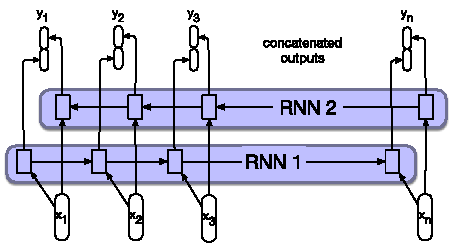
\includegraphics[width=0.45\linewidth]{./img/_birnn.pdf}
\end{figure}

\begin{remark}
    This architecture is not for language modelling (i.e., autoregressive models) as it is assumed that the whole input sequence is available at once.
\end{remark}

\begin{example}[Sequence classification]
    For sequence classification, the last hidden state of the forward and backward contexts can be used as the representation of the whole sequence to pass to the classifier.

    \begin{figure}[H]
        \centering
        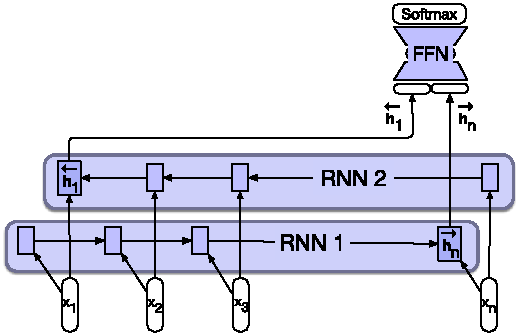
\includegraphics[width=0.35\linewidth]{./img/_birnn_seq_classification.pdf}
    \end{figure}
\end{example}


\subsection{Stacked multi-layer RNN}

\begin{description}
    \item[Stacked RNN] \marginnote{Stacked RNN}
        Stack of RNNs (of any architecture) where:
        \begin{itemize}
            \item The RNN at the first layer $l=1$ processes the input tokens.
            \item The input of any following layer $l \geq 2$ is the hidden state $\vec{h}^{(t)}_{l-1}$ of the previous layer.
        \end{itemize}

        \begin{figure}[H]
            \centering
            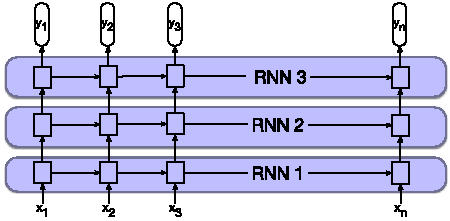
\includegraphics[width=0.45\linewidth]{./img/_layered_rnn.pdf}
        \end{figure}
\end{description}

\begin{remark}
    Skip connections between different layers can help to stabilize the gradient.
\end{remark}



\section{Applications}

\begin{description}
    \item[Autoregressive generation] \marginnote{Autoregressive generation}
        Repeatedly sample a token and feed it back to the network.

        \begin{description}
            \item[Decoding strategy] \marginnote{Decoding strategy}
                Method to select the output token from the output distribution. Possible approaches are:
                \begin{descriptionlist}
                    \item[Greedy] Select the token with the highest probability.
                    \item[Sampling] Randomly sample the token following the probabilities of the output distribution.
                \end{descriptionlist}
        \end{description}

        \begin{description}
            \item[Conditioned generation] \marginnote{Conditioned generation}
                Provide an initial hidden state to the RNN (e.g., speech-to-text).
        \end{description}

    \item[Sequence labeling] \marginnote{Sequence labeling}
        Assign a class to each input token (e.g., POS-tagging, named-entity recognition, structure prediction, \dots).

    \item[Sequence classification] \marginnote{Sequence classification}
        Assign a class to the whole input sequence (e.g., sentiment analysis, document-topic classification, \dots).

    \item[Sentence encoding] \marginnote{Sentence encoding}
        Produce a vector representation for the whole input sequence.
        Possible approaches are:
        \begin{itemize}
            \item Use the final hidden state of the RNN.
            \item Aggregate all the hidden states (e.g., mean).
        \end{itemize}
    
        \begin{example}[Question answering]
            The RNN encoder embeds the question that is used alongside the context (i.e., source from which the answer has to be extracted) to solve a labeling task (i.e., classify each token of the context as non-relevant or relevant).
        \end{example}
\end{description}
